\documentclass[a4paper,11pt]{article}
\usepackage[utf8]{inputenc}
\usepackage[spanish]{babel}
\usepackage[affil-it]{authblk}
\usepackage{enumerate}
\usepackage{graphicx}
\usepackage{hyperref}
\usepackage{amsmath}
\usepackage{amssymb}
\usepackage{cancel}
\usepackage[usenames, dvipsnames]{color}
\usepackage{tikz}
\usepackage[labelfont=bf]{caption}
\usepackage{subcaption} %Multiple images
\usepackage{multicol} % Multiple columns
\usepackage{float}
\usepackage{cleveref}
\usepackage{relsize} % bigger math symbols
\usepackage[margin=1.1in]{geometry}
\usepackage[titletoc,toc,title]{appendix}
\usepackage{enumitem}
\usepackage{etoolbox}
\usepackage{mdframed} %frame theorems
\usetikzlibrary{calc}
\numberwithin{equation}{section}

% Footnotes with symbols

\makeatletter
\def\@fnsymbol#1{\ensuremath{\ifcase#1\or \dagger\or \ddagger\or
   \mathsection\or \mathparagraph\or \|\or **\or \dagger\dagger
   \or \ddagger\ddagger \else\@ctrerr\fi}}
\makeatother

\renewcommand{\thefootnote}{\fnsymbol{footnote}}

% Cool letters 
%Filename:      Typocaps.fd
%Created by:    MLO
%Creation date: 2003/04/02

% This file should be put in a TeX input directory

\ProvidesFile{Typocaps.fd}
   [2003/04/02 Font definition file for U/Typocaps]

\DeclareFontFamily{U}{Typocaps}{}

\DeclareFontShape{U}{Typocaps}{xl}{n}{
   <-> Typocaps
}{}

\endinput


% Footer
\usepackage{fancyhdr}
\pagestyle{fancy}
\fancyhf{}
\cfoot{\fontsize{15pt}{15pt}\usefont{U}{Typocaps}{xl}{n} 
gigantium humeris insidentes}

% Big Pictures
\usepackage[export]{adjustbox}

% Enviroment for theorems
\newmdtheoremenv[frametitle=Teorema]{theo}{Theorem}

% Circled words
\newcommand{\circled}[2][]{%
  \tikz[baseline=(char.base)]{%
    \node[shape = circle, draw, inner sep = 1pt]
    (char) {\phantom{\ifblank{#1}{#2}{#1}}};%
    \node at (char.center) {\makebox[0pt][c]{#2}};}}
\robustify{\circled}

%Appendices in spanish
\renewcommand{\appendixname}{Ap\'endices}
\renewcommand{\appendixtocname}{Ap\'endices}
\renewcommand{\appendixpagename}{Ap\'endices}

%Zero delimiter
\newcommand{\zerodel}{.\kern-\nulldelimiterspace}

%Columns separation
\setlength{\columnsep}{1cm}

%Indentation
\setlength{\parindent}{0ex}

%Multiple References

\crefrangelabelformat{equation}{(#3#1#4--#5\crefstripprefix{#1}{#2}#6)}

\usepackage{xparse}

%Boxes

\newcommand*{\boxcolor}{blue}
\makeatletter
\renewcommand{\boxed}[1]{\textcolor{\boxcolor}{%
\tikz[baseline={([yshift=-1ex]current bounding box.center)}] \node [rectangle, minimum width=1ex,rounded corners,draw] {\normalcolor\m@th$\displaystyle#1$};}}
 \makeatother

%Constantes
\newcommand{\euler}{\mathrm{e}}
\newcommand{\im}{i}

%Lemas, teoremas, definiciones y pruebas
\newcommand{\definicion}{\textbf{Definición: }}
\newcommand{\lema}{\textbf{Lema: }}
\newcommand{\teorema}{\textbf{Teorema: }}
\newcommand{\prueba}{\textbf{Prueba: }}
\newcommand{\proposicion}{\textbf{Proposición: }}
\newcommand{\corolario}{\textbf{Corolario: }}

% Definición de las secciones y su numeración

\makeatletter
\def\@seccntformat#1{%
  \expandafter\ifx\csname c@#1\endcsname\c@section\else
  \csname the#1\endcsname\quad
  \fi}
\makeatother

\begin{document}

\begin{titlepage}
\thispagestyle{fancy}

\newcommand{\HRule}{\rule{\linewidth}{0.5mm}} % Defines a new command for the horizontal lines, change thickness here

\center % Center everything on the page
 
%----------------------------------------------------------------------------------------
%	HEADING SECTIONS
%----------------------------------------------------------------------------------------

\textsc{\LARGE Universidad Nacional Autónoma de México}\\[0.3cm] % Name of your university/college

%----------------------------------------------------------------------------------------
%	LOGO SECTION
%----------------------------------------------------------------------------------------


\includegraphics[scale=0.17]{unam}

%----------------------------------------------------------------------------------------
%	SUBHEADING SECTIONS
%----------------------------------------------------------------------------------------

\textsc{\Large Electrodinámica Clásica}\\[0.3cm] % Major heading such as course name
\textsc{\large Semestre 2016-II}\\[0.3cm] % Minor heading such as course title
\textsc{\large 10 de marzo de 2016}\\ % Minor heading such as course title

%----------------------------------------------------------------------------------------
%	TITLE SECTION
%----------------------------------------------------------------------------------------

\HRule \\[0.1cm]
{ \huge \bfseries Tarea \# 4. \\ Multipolos, Electrostática 
de Medios Macroscópicos, Dieléctricos.}\\ % Title of your document
\HRule \\[0.1cm]
 
%----------------------------------------------------------------------------------------
%	AUTHOR SECTION
%----------------------------------------------------------------------------------------
\setcounter{footnote}{0}
\center
\large
\emph{Autor:} \\ % Your name
\Large Favio \textsc{Vázquez}\footnote[1]{\href{mailto:favio.vazquez@correo.nucleares.unam.mx}{favio.vazquez@correo.nucleares.unam.mx}}

%----------------------------------------------------------------------------------------
%	COOL IMAGE SECTION
%----------------------------------------------------------------------------------------

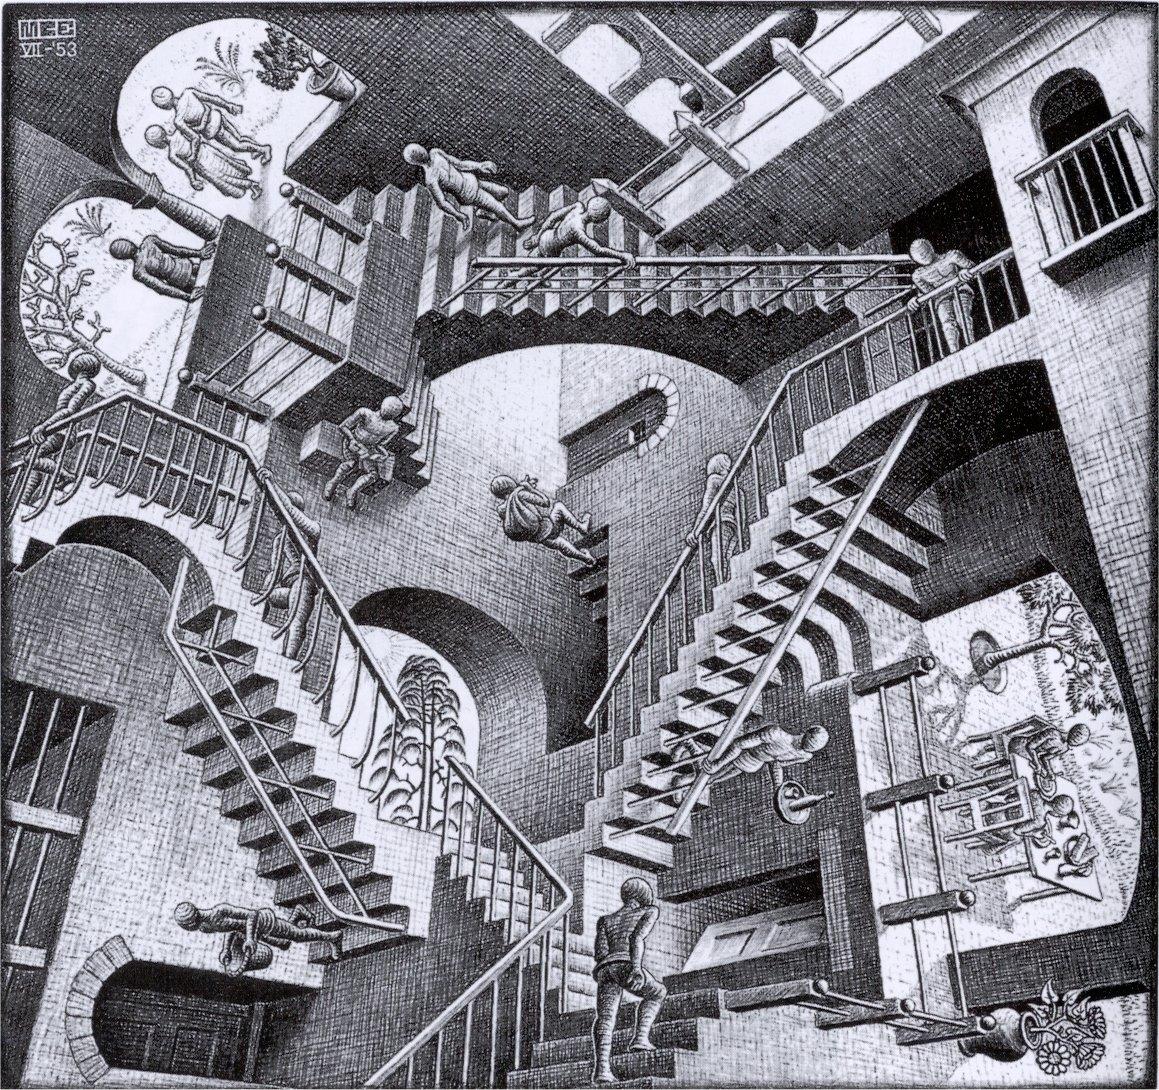
\includegraphics[scale=0.28]{escalerasEscher}

%----------------------------------------------------------------------------------------

\vfill % Fill the rest of the page with whitespace

\end{titlepage}

% ---------------------------------------------------------------------------------------
%         HEADER
%----------------------------------------------------------------------------------------

\fancyhead[L]{Favio Vázquez}
\fancyhead[R]{\thepage}

%----------------------------------------------------------------------------------------
\setcounter{footnote}{0}
\renewcommand*{\thefootnote}{\arabic{footnote}}

\section{Problema 1. Problema 4.1 de Classical Electromagnetic Radiation
de Jackson \cite{jackson}.}

Calcule los momentos multipolares $q_{lm}$ de las distribuciones de carga mostradas 
como las partes $a$ y $b$. Intente obtener resultados para todo los momentos que 
no se hacen cero válidos para todo $l$, pero en cada caso encuentre los primeros 
dos conjuntos de momentos que no se hacen cero al menos.

\begin{figure}[H]
 \center 
 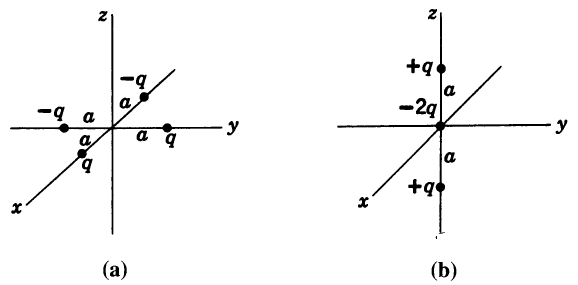
\includegraphics[scale = 0.5]{problema1fig1}
 \caption{Disposición de la distribución de cargas para el problema 1.}
\end{figure}

\begin{enumerate}[label=\textbf{(\alph*)}]
\setcounter{enumi}{2}
\item Para la distribución de carga del segundo conjunto $b$ escriba la expansión 
multipolar para el potencial. Manteniendo solo los términos de orden bajo en la 
expansión, grafique el potencial en el plano $x-y$ como una función de la distancia 
desde el origen para distancias mayores a $a$.
\item Calcule directamente de la ley de Coulomb el potencial exacto para $b$ en 
el plano $x-y$. Grafíquelo como una función de la distancia y compare con el resultados
encontrado en la parte $c$.
\end{enumerate}

Divida la forma asintótica en las partes $c$ y $d$ para ver el comportamiento a 
distancias grandes más claramente.

\vspace{.3cm}

\underline{Solución:} \vspace{.3cm}

Comenzamos recordando la ecuación para los momentos multipolares\footnote{Ver ecuación 
(4.3) de Jackson \cite{jackson}.}

\begin{equation}
 q_{lm} = \sum_i q_ir_i^l Y^*_{lm}(\theta_i,\phi_i),
\end{equation}

donde $(r_i,\theta_i,\phi_i)$ es la posición de la i-ésima carga, $q_i$ es la 
magnitud de la i-ésima carga y $Y^*_{lm}(\theta_i,\phi_i)$ son los armónicos 
esféricos. Viendo la figura de la parte (a) vemos que las cargas, en coordenadas 
esféricas se ubican según la siguiente tabla\footnote{La primera carga es la ubicada 
en $(x=0,y=a,z=0)$}

\begin{table}[H]
\centering
\begin{tabular}{|l|l|l|l|}
\hline
Carga & $r$ & $\theta$ & $\phi$   \\ \hline
$+q$    & $a$ & $\pi/2$  & 0      \\ \hline
$+q$    & $a$ & $\pi/2$  & $\pi/2$  \\ \hline
$-q$    & $a$ & $\pi/2$  & $\pi$    \\ \hline
$-q$    & $a$ & $\pi/2$  & $3\pi/2$ \\ \hline
\end{tabular}
\end{table}

Entonces utilizando esta información tenemos 

\begin{equation}
 q_{lm} = qa^l\left[Y^*_{lm}\left(\frac{\pi}{2},0\right) + 
 Y^*_{lm}\left(\frac{\pi}{2},\frac{\pi}{2}\right) - 
 Y^*_{lm}\left(\frac{\pi}{2},\pi\right) - 
 Y^*_{lm}\left(\frac{\pi}{2},\frac{3\pi}{2}\right)\right].
\end{equation}

Pero recordando que\footnote{Ver ecuación (3.53) y (3.54) de Jackson \cite{jackson}}

\begin{equation}
 Y_{lm}(\theta,\phi) = \sqrt{\frac{2l+1}{4\pi}\frac{(l-m)!}{(l+m)!}}P_l^m(\cos{\theta}) 
 \euler^{im\phi},
 \label{eq:esfericosArmonicosLegendre}
\end{equation}

donde $P_l^m(\cos{\theta}$ son las funciones de Legendre asociadas (ver ecuación 
(3.49) de Jackson) y

\begin{equation}
 Y_{l,-m}(\theta,\phi) = (-1)^m Y^*_{lm}(\theta,\phi), 
\end{equation}

podemos escribir entonces 

\begin{equation*}
 q_{lm} = (-1)^m\sqrt{\frac{2l+1}{4\pi}\frac{(l-m)!}{(l+m)!}} [\euler^{i(-m)(0)} + 
 \euler^{i(-m)(\pi/2)} - \euler^{i(-m)(\pi)} - \euler^{i(-m)(3\pi/2)}] 
 P_l^m(\cancelto{0}{\cos{\frac{\pi}{2}}}),
\end{equation*}

pero 

\begin{align*}
 \euler^{i(-m)(0)} &= 1, \\
 \euler^{i(-m)(\pi/2)} &= (\euler^{-i\pi/2})^{(m)} = (-i)^m, \\
 \euler^{i(-m)(\pi)} &= (\euler^{-i\pi})^{(m)} = (-1)^m, \\
 \euler^{i(-m)(3\pi/2)} &= (\euler^{-i3\pi/2})^{(m)} = i^m.
\end{align*}

Tenemos entonces, 

\begin{equation}
 q_{lm} = qa^l\sqrt{\frac{2l+1}{4\pi}\frac{(l-m)!}{(l+m)!}}\left[1 + 
 (-i)^m - (-1)^m - i^m \right]P_l^m(0),
\end{equation}

el término entre corchetes $\left[1 +  (-i)^m - (-1)^m - i^m \right]$ es cero 
para $m$ par, y se hace $(2-2i)$ para $m = -7,-3,1,5,9,\dots$ y $(2+2i)$ para 
$m=-5,-1,3,7,\dots$, además por las propiedades de $P_l^m(0)$ sabemos que se 
hace cero cuando $l$ y $m$ tienen signos diferentes. Estas dos consideraciones 
no hacen ver que los únicos momentos que no se hacen cero son aquellos con 
$l$ y $m$ impares. Y como el texto lo solicita, los primeros conjuntos de momentos 
que no se hacen cero son 

\begin{equation}
 \boxed{q_{1,\pm 1} = \mp qa\sqrt{\frac{3}{4\pi}} (1 \mp i)},
\end{equation}

\begin{equation}
 \boxed{q_{3,\pm 1} = \pm qa^3\sqrt{\frac{21}{\pi}} (1 \mp i)},
\end{equation}

\begin{equation}
 \boxed{q_{3,\pm 3} = \mp qa^3\sqrt{\frac{35}{16\pi}} (1 \pm i)},
\end{equation}

\newpage

\textbf{(b)} Viendo la figura de la parte (b) vemos que las cargas, en coordenadas 
esféricas se ubican según la siguiente tabla\footnote{La primera carga es la ubicada 
en $(x=0,y=0,z=a)$}

\begin{table}[H]
\centering
\begin{tabular}{|l|l|l|l|}
\hline
Carga 	& $r$ & $\theta$ & $\phi$   \\ \hline
$+q$    & $a$ & $0$ 	 & $0$      \\ \hline
$-2q$   & $0$ & $0$	 & $0$  \\ \hline
$+q$    & $a$ & $\pi$  	 & $0$    \\ \hline
\end{tabular}
\end{table}

Entonces, 

\begin{equation}
 q_{lm} = q\left[a^lY^*_{lm}(0,0) - \cancelto{0}{(0)^l lY^*_{lm}(0,0)} + 
 a^llY^*_{lm}(\pi,0)\right],
\end{equation}

y usando \eqref{eq:esfericosArmonicosLegendre} podemos escribir esto como 

\begin{equation}
 q_{lm} = qa^l\sqrt{\frac{2l+1}{4\pi}\frac{(l-m)!}{(l+m)!}} 
 \left[ e^{im(0)}P_l^m(\cos(0)) + e^{im(0)}P_l^m(\cos(\pi)) \right],
\end{equation}

\begin{equation}
 \therefore q_{lm}qa^l\sqrt{\frac{2l+1}{4\pi}\frac{(l-m)!}{(l+m)!}} 
 \left[P_l^m(1) + P_l^m(-1) \right].
\end{equation}

Debido a que el sistema tiene simetría azimutal, solamente los términos con 
$m=0$ serán distintos de cero, y notando que $P_l^0(1) = 1, P_l^0(-1) = (-1)^l$ 
tenemos que 

\begin{equation}
 q_{l0} = qa^l\left[\frac{2l+1}{4\pi} \right]^{1/2}[1 + (-1)^l],
\end{equation}

y tendremos que para $l$ par y $m=0$, 

\begin{equation}
 q_{l0} = 2qa^l\left[\frac{2l+1}{4\pi} \right],
 \label{eq:momentoCasoB}
\end{equation}

y para $l$ impar o $m \neq 0$ $q_{l0} = 0$. Los primeros momentos que 
no se hacen cero son 

\begin{equation}
 \boxed{q_{2,0} = qa^2\sqrt{\frac{5}{\pi}}},
\end{equation}

\begin{equation}
 \boxed{q_{4,0} = qa^4\sqrt{\frac{9}{\pi}}}.
\end{equation}

\textbf{(c)} La expansión multipolar para el potencial podemos escribirla como\footnote{Ver 
ecuación (4.1) de Jackson \cite{jackson}.} 

\begin{equation}
 \Phi(r,\theta,\phi) = \frac{1}{4\pi\epsilon_0 r}\sum_{l=0}^\infty 
 \sum_{m=-l}^l \frac{4\pi}{2l+1} 
 q_{lm} \frac{Y_{lm}(\theta,\phi)}{r^{l+1}},
\end{equation}

y sustituyendo \eqref{eq:momentoCasoB} obtenemos 

\begin{equation}
 \Phi(r,\theta,\phi) = \frac{1}{4\pi\epsilon_0}\sum_{l=1}^\infty \frac{4\pi}{2l+1}  
 \left(qa^{2l}\sqrt{\frac{(4l+1)}{4\pi}} \right)\frac{Y_{2l,0}(\theta,\phi)}{r^{2l+1}},
\end{equation}

\begin{equation}
 \boxed{\Phi(r,\theta) = \frac{q}{2\pi\epsilon_0 r}\sum_{l=1}P_{2l}(\cos{\theta})
 \left(\frac{a}{r}\right)^{2l}}.
\end{equation}

El término de orden más bajo se da cuando $l=1$, 

\begin{equation}
 \Phi(r,\theta) = \frac{q}{4\pi\epsilon_0}\frac{a^2}{r^3}\left[ 
 \frac{1}{2}(3\cos^2{\theta} - 1)\right],
\end{equation}

que en el plano $x-y$, donde $\theta = \pi/2$ tenemos 

\begin{equation}
 \Phi_{x-y}(r,\theta) = - \frac{q}{8\pi\epsilon_0}\frac{a^2}{r^3}.
\end{equation}

Cuyo gráfico es 

\begin{figure}[H]
\center 
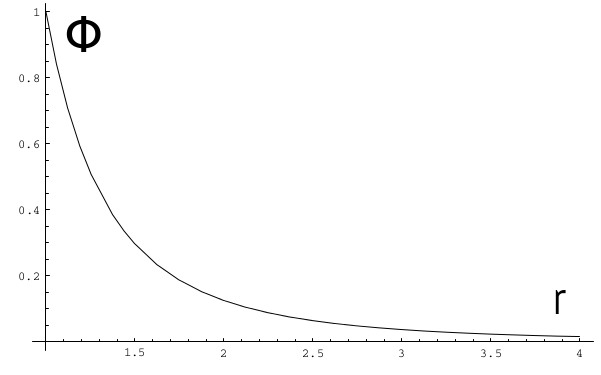
\includegraphics[scale=0.6]{problema1fig2}
\caption{Gráfico del potencial aproximado utilizando expansión multipolar 
para términos de orden bajo en el plano $x-y$.}
\end{figure}

\textbf{(d)} Utilizando la ley de Coulomb podemos escribir el potencial como

\begin{align*}
 \Phi = \frac{1}{4\pi\epsilon_0}\left[\frac{1}{|\mathbf{r} + a\hat{\mathbf{z}}|}
 \frac{1}{|\mathbf{r} - a\hat{\mathbf{z}}|} - \frac{2}{|\mathbf{r}|} \right],
\end{align*}

que en el plano $x-y$ se escribe 

\begin{equation}
 \Phi = \frac{2q}{4\pi\epsilon_0}\left[\frac{1}{\sqrt{r^2+a^2}} - \frac{1}{r} \right],
\end{equation}

o 

\begin{equation}
 \boxed{\Phi = \frac{q}{4\pi\epsilon_0 a}\left[\frac{2}{\sqrt{(r/a)^2 + 1}} - 
 \frac{2}{(r/a)}\right]}.
\end{equation}

\newpage

Cuyo gráfico es 

\begin{figure}[H]
\center 
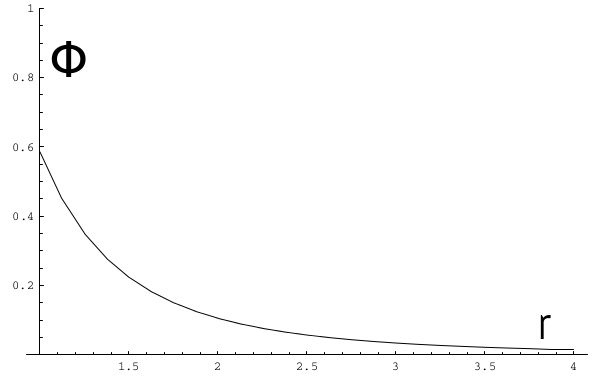
\includegraphics[scale=0.6]{problema1fig3}
\caption{Gráfico del potencial exacto, en el plano $x-y$,
utilizando la ley de Coulomb}
\end{figure}

Con lo cual vemos que el primer término en la expansión multipolar es una buena 
aproximación para distancias $r \approx 2a$, pero impreciso para otras más pequeñas.

\vspace{.3cm}

Si dividimos ahora la forma asintótica en las partes (c) y (d) para ver el comportamiento 
a distancias grandes, lo que tenemos que hacer es dividir por $1/r^3$ tanto 
el potencial aproximado como el exacto, obteniendo el siguiente gráfico

\begin{figure}[H]
\center 
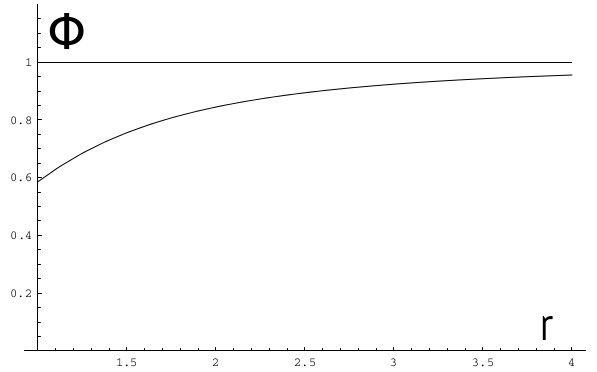
\includegraphics[scale=0.6]{problema1fig4}
\caption{Comportamiento del potencial tanto para la forma aproximada como para 
la exacta, donde se ha dividido la forma asintótica. La línea recta es la aproximación 
de la parte (c) y la otra es la obtenida con la ley de Coulomb en la parte (d).}
\end{figure}

Vemos que la aproximación mejora para $r \gg a$. 

\newpage

\section{Problema 2. Problema 4.7 de Classical Electromagnetic Radiation
de Jackson \cite{jackson}.}

Una distribución de carga localizada tiene la densidad de carga 

$$
\rho(\mathbf{r}) = \frac{1}{64\pi}r^2\euler^{-r}\sen^2{\theta}
$$

\begin{enumerate}[label=\textbf{(\alph*)}]
\item Haga una expansión multipolar del potencial debido a esta densidad de 
carga y determine todos los momentos multipolares que no se hacen cero. Escriba 
el potencial a grandes distancias como una expansión finita en polinomios de 
Legendre. 
\item Determine el potencial explícitamente en cualquier punto del espacio, y 
muestre que cerca del origen, correcto a $r^2$ inclusive,

$$
\Phi(\mathbf{r}) \simeq \frac{1}{4\pi\epsilon_0}\left[\frac{1}{4} 
 - \frac{r^2}{120}P_2(\cos{\theta})\right]
$$

\item Si existe en el origen un núcleo con un momento cuadrupolar $Q = 10^{-28}$ m$^2$, 
determine la magnitud de la energía de interacción, asumiendo que la unidad de 
carga en $\rho(\mathbf{r})$ arriba es la carga electrónica y que la unidad de 
longitud es el radio de Bohr del hidrógeno $a_0 = 4\pi\epsilon_0\hslash/me^2 = 
0.529 \times 10^{-10}$ m. Exprese su respuesta como una frecuencia dividida por 
la constante de Planck $h$.
\end{enumerate}

La densidad de carga en este problema es la de los estados $m = \pm 1$ del nivel 
$2p$ en el hidrógeno, mientras que la interacción cuadrupolar es del mismo orden 
que el encontrado en moléculas.

\vspace{.3cm}

\underline{Solución:} \vspace{.3cm}

\textbf{(a)} Recordando que la expresión integral para los momentos multipolares es 

\begin{equation}
 q_{lm} = \int \rho(r',\theta',\phi')r'^l Y^*_{lm}(\theta',\phi')dV',
\end{equation}

y debido a que no hay dependencia en $\phi$ en el problema, solo serán distintos de 
cero los momentos con $m=0$. Tenemos entonces\footnote{Ver el problema anterior 
para una referencia sobre la relación entre los armónicos esféricos y los polinomios 
de Legendre.} (ver ecuación (3.57) de Jackson \cite{jackson})

\begin{equation}
 q_{l0} = \frac{1}{64\pi}\sqrt{\frac{2l+1}{4\pi}}\int_0^\infty \int_0^\pi \int_0^{2\pi} 
 r^{l+4}\euler^{-r}\sen^3{\theta}P_l(\cos{\theta})drd\theta d\phi
\end{equation}

que por propiedades de los polinomios de Legendre\footnote{Ver sección 3.3 de 
Jackson \cite{jackson}.}

\begin{equation}
 q_{l0} = \frac{1}{32}\sqrt{\frac{2l+1}{4\pi}}\left[\int_0^\infty r^{l+4}e^{-r} dr \right]
 \left[\int_{-1}^1 (1-x^2)P_l(x)dx \right],
\end{equation}

La segunda integral puede escribirse como 

\begin{equation}
 \int_{-1}^1 (1-x^2)P_l(x)dx = \int_{-1}^1 P_l(x)dx - \int_{-1}^1 x^2P_l(x)dx,
\end{equation}

y por la ortogonalidad de los polinomios de Legendre vemos que la primera integral 
no es cero solamente para $l=0$ y por lo tanto será igual a 2, y para la segunda
integral podemos usar la ecuación 3.32 de Jackson \cite{jackson} que nos dice 
que esta integral tendrá un valor de $2/3$ para $l=0$, $4/15$ para $l=2$ y será 
cero para cualquier otro valor de $l$. Por lo tanto 

\begin{equation}
 \int_{-1}^1 (1-x^2)P_l(x)dx = \begin{cases}
				 \frac{4}{3}, \quad  \qquad l=0 \\
				 -\frac{5}{15}, \quad \quad l=2 \\
				 0 \quad \qquad \text{de otra manera}.
				\end{cases}
\end{equation}

Entonces solo necesitamos evaluar la otra integral para $l=0$ y $l=2$, y de 
tablas de integrales vemos que\footnote{\href{http://1.usa.gov/1TxNpSt}{http://1.usa.gov/1TxNpSt}}

\begin{equation}
 \int_0^\infty r^n \euler^{-r}dr = n!,
\end{equation}

\begin{equation}
\therefore \int_0^\infty r^{l+4} \euler^{-r}dr = (l+4)!
\end{equation}

y tenemos entonces 

\begin{equation}
 \int_0^\infty r^{l+4} \euler^{-r}dr = \begin{cases}
				    24, \hspace{.8cm} l=0 \\
				    720, \hspace{.6cm} l=2.
				\end{cases}
\end{equation}

Y utilizando estos resultados encontramos que los momentos multipolares 
que no se hacen cero son 

\begin{equation}
 \boxed{q_{00} = \sqrt{\frac{1}{4\pi}}}.
\end{equation}

\begin{equation}
 \boxed{q_{20} = -6 \sqrt{\frac{5}{4\pi}}}.
\end{equation}

Ahora, la expansión multipolar del potencial podemos escribirla como\footnote{Ver 
ecuación (4.1) de Jackson \cite{jackson}.}

\begin{equation}
  \Phi(r,\theta,\phi) = \frac{1}{4\pi\epsilon_0 r}\sum_{l=0}^\infty 
 \sum_{m=-l}^l \frac{4\pi}{2l+1} 
 q_{lm} \frac{Y_{lm}(\theta,\phi)}{r^{l+1}},
\end{equation}

que con los momentos multipolares que hemos encontrado puede escribirse como 

\begin{equation}
  \Phi(r,\theta) = \frac{1}{4\pi\epsilon_0}\left[\frac{1}{r} - 
  \frac{6}{r^3}P_2(\cos{\theta})  \right]
\end{equation}

\begin{equation}
 \boxed{\therefore \Phi(r,\theta) = \frac{1}{4\pi\epsilon_0 r}\left[1 - 
  \frac{6}{r^2}P_2(\cos{\theta})\right]}.
\end{equation}

\textbf{(b)} La forma explícita para el potencial en cualquier punto del 
espacio la calculamos con 

\begin{equation}
 \Phi(\mathbf{x}) = \frac{1}{4\pi\epsilon_0} \int \frac{\rho(\mathbf{r}'}{|\mathbf{x} - 
 \mathbf{x}'|}d\mathbf{x}',
\end{equation}

expandiendo el término $1/|\mathbf{x} -  \mathbf{x}'|$ en armónicos esféricos y usando 
la diferencial de volumen en coordenadas esféricas podemos escribir (usando la notación 
de Jackson \cite{jackson})

\begin{equation}
 \Phi(\mathbf{x}) = \frac{1}{64\pi \epsilon_0 }\sum_{lm} \frac{1}{2l+1}Y_{lm}(\theta,\phi) 
 \left[\int \frac{r^l_{<}}{r^{l+1}_{>}}r'^4\euler^{-r'} dr\right]
 \left[\int Y^*_{lm}(\theta',\phi')\sen^3{\theta'}d\theta' d\phi' \right],
\end{equation}

\begin{equation}
 \therefore \Phi(\mathbf{x}) = \frac{1}{128\pi \epsilon_0 }\sum_l P_l(\cos{\theta})
 \left[\int \frac{r^l_{<}}{r^{l+1}_{>}}r'^4\euler^{-r'} dr\right]
 \left[\int_{-1}^1 (1-x^2)P_l(x)dx\right].
\end{equation}

De nuevo como arriba, todos los términos con $m \neq 0$ serán cero. Ya hemos resuelto 
la integral de la derecha, y sustituyendo estos valores encontramos que\footnote{Utilizando 
una muy inteligente notación de \href{http://homerreid.dyndns.org/physics/jackson/}{http://homerreid.dyndns.org/physics/jackson/}}

\begin{equation}
 \boxed{\Phi(\mathbf{x}) = \frac{1}{128}\left[\frac{4}{3}\xi_0 - \frac{4}{15}\xi_2 
 P_2(\cos{\theta})\right]},
\end{equation}

donde $xi_l$ se refiere a la integral en $r'$. Esta integral solo debe evaluarse 
para $l=0$ y para $l=2$. Para el caso en que $l=0$ tenemos 

\begin{equation}
 \xi_0 = \frac{1}{r}\int_0^r r'^4 \euler^{-r'} dr' + \int_r^\infty r'^3\euler^{-r'} dr',
\end{equation}

\begin{equation}
 \boxed{\xi_0 = \frac{1}{r}[24 - \euler^{-r}(r^3 + 6r^2 + 18r + 24)]},
\end{equation}

y para el caso en que $l=2$ tenemos 

\begin{equation}
  \xi_2 = \frac{1}{r^3}\int_0^r r'^6 \euler^{-r'} dr' + r^2 \int_r^\infty r'\euler^{-r'} dr',
\end{equation}

\begin{equation*}
 \boxed{\xi_2 = \frac{1}{r^3}[720 - \euler^{-r}(r^6 + 6r^5 + 30r^4 + 120r^3 + 360r^4 + 
 720r + 720)] + r^2[\euler^{-r}(1-r)]}
\end{equation*}

Lo cual completa el cálculo del potencial en cualquier punto del espacio. Ahora cerca 
del origen, es decir cuando $r \rightarrow 0$ tenemos 

\begin{equation}
 \xi_0 \simeq 6, \qquad \quad \xi_2 \simeq r^2 - 2r^3 + \frac{3}{2}r^4.
\end{equation}

Por lo tanto al sustituir estas expresiones en la ecuación que encontramos para el 
potencial en todo punto del espacio encontramos 

\begin{equation}
 \boxed{\Phi(\mathbf{x}) = \frac{1}{4\pi\epsilon_0}\left[\frac{1}{4} - \frac{r^2}{120} 
 P_2(\cos{\theta})\right]}.
\end{equation}

\hspace{10cm}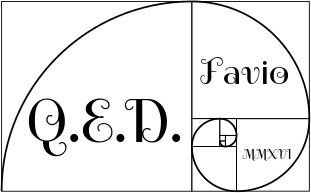
\includegraphics[scale=0.25]{logoQED}

\textbf{(c)} La energía de la interacción cuadrupolar está dada por el tercer término
de la ecuación (4.24) de Jackson \cite{jackson}, 

\begin{equation}
 W^(4) = -\frac{1}{6}\sum_{ij} Q_{ij} \left\zerodel\frac{\partial E_j}{\partial x_i}
 \right|_{x=0},
\end{equation}

además para un núcleo atómico tenemos simetría en el eje $z$ (eje arbitrario), por 
lo tanto se cumple que\footnote{Ver ecuación (2.38) de Marion y Heald \cite{marion2}.} 

\begin{equation}
 Q_{33} = - 2Q_{11} = - 2Q_{22} = eQ,
\end{equation}

y todos las demás componentes son cero. Y entonces 

\begin{equation}
 W = \frac{eQ}{6}\left|\frac{1}{2}\frac{\partial E_x}{\partial x} + 
 \frac{1}{2}\frac{\partial E_y}{\partial y} - \frac{\partial E_z}{\partial z}
 \right|_{\mathbf{x}=0}, 
\end{equation}

que podemos escribir como 

\begin{equation}
 W = \frac{eQ}{6}\left|\frac{1}{2}\nabla \cdot \mathbf{E} 
 - \frac{3}{2}\frac{\partial E_z}{\partial z}\right|_{\mathbf{x}=0},
\end{equation}

y utilizando la ley de Gauss encontramos 

\begin{equation}
  W = \frac{eQ}{6}\left|\frac{1}{2}\frac{\cancelto{0}{\rho}}{\epsilon_0}
 - \frac{3}{2}\frac{\partial E_z}{\partial z}\right|_{\mathbf{x}=0},
\end{equation}

donde recordamos que $\rho \rightarrow 0$ en el origen. Tenemos entonces 

\begin{equation}
 W = - \frac{eQ}{4}\left|\frac{\partial E_z}{\partial z} \right|_{\mathbf{x}=0},
\end{equation}

\begin{equation}
 \therefore W = -\frac{eQ}{4}\left|\frac{\partial^2 \Phi}{\partial z^2} \right|_{\mathbf{x}=0}.
\end{equation}

Para calcular esta última derivada parcial necesitamos expresar el potencial obtenido 
en el inciso anterior en coordenadas cartesianas, que ignorando la parte constante 
podemos escribir como 

\begin{equation}
 \Phi(\mathbf{x}) = \frac{1}{480\pi\epsilon_0}r^2P_2(\cos{\theta}),
\end{equation}

\begin{equation}
  \Phi(\mathbf{x}) = \frac{1}{960\pi\epsilon_0}r^2(3\cos{\theta} - 1),
\end{equation}

usando la definición de $r$ y de $\cos{\theta}$

\begin{equation}
  \therefore \Phi(\mathbf{x}) = \frac{1}{960\pi\epsilon_0}(2z^2 - x^2 - y^2),
\end{equation}

y diferenciando obtenemos 

\begin{equation}
 \frac{\partial^2 \Phi}{\partial z^2} = \frac{1}{240\pi\epsilon_0},
\end{equation}

y sustituyendo este resultado en la ecuación para $W$ obtenemos 

\begin{equation}
 W = \frac{eQ}{960\pi\epsilon_0},
\end{equation}

ahora para asegurar que las dimensiones están correctas debemos multiplicar por 
$e$ y dividir por $a_0^3$, obtenemos entonces 

\begin{equation}
 \frac{W}{\hbar} = \frac{1}{240}\frac{e^2Q}{4\pi\epsilon_0\hbar a_0^3},
\end{equation}

que podemos escribir como\footnote{Utilizando la ecuación para la constante 
de estructura fina $\alpha = \frac{1}{4\pi\epsilon_0}\frac{e^2}{\hbar c}$.}

\begin{equation}
 \frac{W}{\hbar} = \frac{1}{240}\frac{\alpha c Q}{a_0^3},
\end{equation}

y sustituyendo los valores que nos da el texto encontramos 

\begin{equation}
 \boxed{\frac{W}{\hbar} = 6.16 \times 10^6 \text{ rad/s} \simeq 1 \text{ MHz}}.
\end{equation}

\newpage

\section{Problema 3. Problema 4.8 de Classical Electromagnetic Radiation
de Jackson \cite{jackson}.}

Un cascarón cilíndrico, muy largo y circular recto, de constante dieléctrica 
$\epsilon/\epsilon_0$ y radio interno y externo $a$ y $b$, respectivamente, 
es colocado en un previamente campo eléctrico uniforme $E_0$ con su eje perpendicular 
al campo. El medio adentro y afuera del cilindro tiene una constante dieléctrica de 
uno.

\begin{enumerate}[label=\textbf{(\alph*)}]
\item Determine el potencial y campo eléctrico en las tres regiones, despreciando 
efectos finales.
\item Esboce las líneas de fuerza para un caso típico de $b \simeq 2a$.
\item Discuta las formas limitantes en su solución apropiadas para un cilindro 
dieléctrico sólido en un campo uniforme, y una cavidad cilíndrica en un dieléctrico 
uniforme.
\end{enumerate}

\vspace{.3cm}

\underline{Solución:} \vspace{.3cm}

Debido a que el cilindro es muy largo y uniforme sobre su eje, y el campo original 
es también uniforme, el problema puede reducirse a dos dimensiones, y por la simetría 
del mismo trabajaremos en coordenadas polares. Supongamos además que el campo apunta 
hacia el lado positivo del eje $x$. 

\vspace{.3cm}

Por otra parte, ya que no hay carga libre en ningún lado, y además no hay carga ligada 
en ningún lado excepto la superficie del cilindro, podemos dividir el problema en 
tres regiones, y usar la solución a la respectiva ecuación de Laplace en cada 
región.

\vspace{.3cm}

Recordemos que la solución general de la ecuación de Laplace en coordenadas polares
cuando se trabaja con un barrido angular total es\footnote{Ver ecuación (2.71) de 
Jackson \cite{jackson}.}

\begin{equation}
 \Phi(\rho,\phi) = a_0 + b_0 \ln{\rho} + \sum_{m=1}^\infty (a_m \rho^m + b_m \rho^{-m})
 (A_m \euler^{im\phi} + B_m \euler^{-im\phi}).
\end{equation}

La región interna incluye el origen, por lo que debe tener la forma 

\begin{equation}
 \boxed{\Phi_{\rho < a} = \sum_{m=0}^\infty \rho^m (A_m \euler^{im\phi} + B_m \euler^{-im\phi})}.
\end{equation}

La región externa debe comportarse como un campo uniforme a distancias grandes, entonces 
recordando que hemos escogido que el campo apunta hacia el lado positivo del eje $x$

\begin{equation}
 - E_0\rho\cos{\phi} =  a_0 + b_0 \ln{\rho} + \sum_{m=1}^\infty (a_m \rho^m + b_m \rho^{-m})
 (A_m \euler^{im\phi} + B_m \euler^{-im\phi}),
\end{equation}

debido a la ortogonalidad tenemos que $a_0 = 0$, $b_0 = 0$, y solo el término con 
$m=1$ no se hace cero, y $A_1 = B_1$, entonces 

\begin{equation}
 -E_0 = a_1 2 B_1,
\end{equation}

por lo que la solución se convierte en 

\begin{equation}
 \boxed{\Phi_{\rho>b} = (-E_0 \rho + b_1 \rho^{1})\cos{\theta}}.
\end{equation}

La región del medio simplemente conecta las otras dos regiones, 

\begin{equation}
 \boxed{\therefore \Phi_{a < \rho < b} = c_0 + d_0 \ln{\rho} + \sum_{m=1}^\infty (c_m \rho^m + d_m \rho^{-m})
 (C_m \euler^{im\phi} + D_m \euler^{-im\phi})}.
\end{equation}

Debemos ahora calcular estos parámetros que hemos puesto a lo largo de las expresiones 
para los potenciales; para hacer esto partimos de las condiciones de frontera que 
deben cumplirse, i.e.

\begin{equation}
 (\epsilon_2 \mathbf{E}_2 - \epsilon_1 \mathbf{E}_1)\cdot \mathbf{n} = \sigma,
\end{equation}

pero debido a que no hay carga libre y que el campo eléctrico se propaga la dirección 
radial tenemos 

\begin{equation}
  \epsilon_2 \mathbf{E}_2 \cdot \hat{\rho} =
  \epsilon_1 \mathbf{E}_1 \cdot \hat{\rho}.
\end{equation}

Aplicando esto a la superficie exterior ($\rho = b$) obtenemos

\begin{equation}
 \epsilon_0 \left\zerodel\frac{\partial \Phi_{\rho>b}}{\partial \rho}\right|_{\rho=b} = 
 \epsilon \left\zerodel\frac{\partial \Phi_{a < \rho < b}}{\partial \rho}\right|_{\rho=b},
\end{equation}

\begin{align*}
 \epsilon_0 \left\zerodel\frac{\partial}{\partial \rho}\left[ (-E_0 \rho + b_1 \rho^{1})\cos{\phi}
 \right]\right|_{\rho=b} &= \epsilon \frac{\partial}{\partial \rho} \left[c_0 + d_0 \ln{\rho}\right\zerodel \\
 &+ \left\zerodel\sum_{m=1}^\infty (c_m \rho^m + d_m \rho^{-m})
 (C_m \euler^{im\phi} + D_m \euler^{-im\phi})]\right|_{\rho=b},
\end{align*}

\begin{equation*}
 \therefore \epsilon_0\left[(-E_0 - b_1b^{-2})\cos{\phi}\right] = 
 \epsilon \left[ d_0 \frac{1}{b} + \sum_{m=1}^\infty(c_m m b^{m-1} - 
 m d_m b^{-m-1})(C_m \euler^{im\phi} + D_m \euler^{-im\phi})\right].
\end{equation*}

Debido a la ortogonalidad encontramos que $d_0 = 0$, $D_m = C_m$ y solamente se 
mantienen los términos con $m=1$; también podemos despreciar el $c_0$ ya que es 
una constante que no afecta el resultado final, entonces 

\begin{equation}
 \epsilon_0\left[(-E_0 - b_1b^{-2})\cos{\phi}\right] = 
 \epsilon [(c_1 - d_1 b^{-2})C_1 2\cos{\phi}),
\end{equation}

combinando ahora los factores de $c_1$ con $C_1$ encontramos 

\begin{equation}
 C_1 = \frac{-\epsilon_0(-E_0 - b_1b^{-2})}{2\epsilon(1 - d_1b^{-2}},
\end{equation}

y la solución del medio se convierte por ahora en 

\begin{equation}
 \Phi_{a < \rho < b} = -(\rho + d_1 \rho^{-1})
 \frac{-\epsilon_0(-E_0 - b_1b^{-2})}{2\epsilon(1 - d_1b^{-2}}\cos{\phi}.
\end{equation}

Aplicando la otra condición de frontera en la superficie exterior ($\rho = b$) 

\begin{equation}
 \left\zerodel E_{r,2}\right|_{\rho=b} = \left\zerodel E_{r,1}\right|_{\rho=b},
\end{equation}

\begin{equation*}
 \left\zerodel\frac{\partial \Phi_{\rho>b}}{\partial \phi}\right|_{\rho=b} = 
 \left\zerodel\frac{\partial \Phi_{a < \rho < b}}{\partial \phi}\right|_{\rho=b},
\end{equation*}

\begin{equation*}
 \left\zerodel\frac{\partial}{\partial \phi}\left[(-E_0 \rho + b_1 \rho^{1})\cos{\phi} \right]\right|_{\rho=b} = 
\left\zerodel \frac{\partial}{\partial \phi}\left[c_0  -(\rho + d_1 \rho^{-1})
 \frac{-\epsilon_0(-E_0 - b_1b^{-2})}{2\epsilon(1 - d_1b^{-2}}\cos{\phi}\right]\right|_{\rho=b}
\end{equation*}

\begin{equation}
 \therefore (E_0 - b_1b^{-2})\epsilon(1 - d_1 b^{-2}) = (1 + d_1b^{-2})\epsilon_0 
 (E_0+ b_1b^{-2}),
\end{equation}

y entonces 

\begin{equation}
 d_1 = b^2 \frac{b_1(\epsilon + \epsilon_0) - E_0b^2(\epsilon - \epsilon_0)}
 {b_1(\epsilon - \epsilon_0) - E_0b^2(\epsilon + \epsilon_0)},
\end{equation}

y la solución en la región central se convierte en 

\begin{equation*}
 \boxed{\Phi_{a < \rho < b} = \frac{1}{2\epsilon b^2}\cos{\phi}\left\{
 b_1(\epsilon - \epsilon_0) - E_0 b^2 (\epsilon + \epsilon_0)\rho 
 + b^2[(b_1(\epsilon+\epsilon_0) - E_0 b^2(\epsilon - \epsilon_0)\rho^{-1}]\right\}}.
\end{equation*}

Ahora aplicando las condiciones de frontera en la superficie interna $(\rho = a)$ 

\begin{equation}
  \epsilon_0 \left\zerodel\frac{\partial \Phi_{\rho>b}}{\partial \rho}\right|_{\rho=a} = 
 \epsilon \left\zerodel\frac{\partial \Phi_{a < \rho < b}}{\partial \rho}\right|_{\rho=a},
\end{equation}

obtenemos 

\begin{equation}
 \frac{1}{2b^2}\left\{
 b_1(\epsilon - \epsilon_0) - E_0 b^2 (\epsilon + \epsilon_0) 
 + b^2[(b_1(\epsilon+\epsilon_0) - E_0 b^2(\epsilon - \epsilon_0)]a^{-2}\right\} = 
 \epsilon_0 A_1,
\end{equation}

y 

\begin{equation}
 \left\zerodel\frac{\partial \Phi_{\rho>b}}{\partial \phi}\right|_{\rho=a} = 
 \left\zerodel\frac{\partial \Phi_{a < \rho < b}}{\partial \phi}\right|_{\rho=a},
\end{equation}

obtenemos 

\begin{equation}
 \frac{1}{2\epsilon a b^2}\left\{
 [b_1(\epsilon - \epsilon_0) - E_0 b^2 (\epsilon + \epsilon_0)]a 
 + b^2[(b_1(\epsilon+\epsilon_0) - E_0 b^2(\epsilon - \epsilon_0)]a^{-1}\right\} = 
 A_1,
\end{equation}

Y resolviendo este sistema de ecuaciones con \texttt{Mathematica$^\circledR$} obtenemos 

\begin{equation}
 b_1 = E_0 b^2 \frac{(b^2 - a^2)(\epsilon^2 - \epsilon_0^2)}{b^2(\epsilon + 
 \epsilon_0)^2 - a^2(\epsilon - \epsilon_0)^2}, 
\end{equation}

y 

\begin{equation}
 A_1 = - \frac{4b^2 E_0 \epsilon \epsilon_0}{b^2(\epsilon + \epsilon_0)^2 
 - a^2(\epsilon - \epsilon_0)^2}.
\end{equation}

Ya tenemos todos los parámetros que necesitamos para escribir las expresiones que 
encontramos arriba para los potenciales en las tres regiones, que resultan 

\begin{equation}
 \boxed{\Phi_{\rho < a} = E_0\rho\cos{\phi} \left[- \frac{4b^2 E_0 \epsilon
 \epsilon_0}{b^2(\epsilon + \epsilon_0)^2 
 - a^2(\epsilon - \epsilon_0)^2} \right]},
\end{equation}

\begin{equation}
 \boxed{\Phi_{a < \rho < b} = \frac{-2ab^2\epsilon_0}{b^2(\epsilon + \epsilon_0)^2 
 - a^2(\epsilon - \epsilon_0)^2}\left[(\epsilon + \epsilon_0)\frac{\rho}{a} 
 + (\epsilon + \epsilon_0)\frac{a}{\rho}\right]E_0\cos{\phi}},
\end{equation}

\begin{equation}
 \boxed{\Phi_{\rho>b} = E_0\cos{\phi}\left[-\rho + \frac{(b^2 - a^2)(\epsilon^2 -
 \epsilon_0^2)}{b^2(\epsilon +  \epsilon_0)^2 - a^2(\epsilon - \epsilon_0)^2} 
 \frac{b^2}{\rho}\right]}.
\end{equation}

Para obtener los campos eléctricos utilizamos

\begin{equation}
 \mathbf{E} = -\hat{\rho}\frac{\partial \Phi}{\partial \rho} 
 - \hat{\phi}\frac{1}{\rho}\frac{\partial \Phi}{\partial \phi},
\end{equation}

y luego de hacer las derivadas y un poco de álgebra, recordando la 
dirección del campo eléctrico que hemos escogido, obtenemos 

\begin{equation}
 \boxed{\mathbf{E}_{\rho < a} = E_0 \left[- \frac{4b^2 E_0 \epsilon
 \epsilon_0}{b^2(\epsilon + \epsilon_0)^2 
 - a^2(\epsilon - \epsilon_0)^2} \right]\hat{i}},
\end{equation}

\begin{equation}
 \boxed{\mathbf{E}_{a < \rho < b} = \frac{2ab^2\epsilon_0E_0}{b^2(\epsilon + \epsilon_0)^2 
 - a^2(\epsilon - \epsilon_0)^2}\left[(\epsilon + \epsilon_0)\hat{i}
 - (\epsilon - \epsilon_0)\frac{a^2}{\rho^2}(\hat{i} + 2\hat{\phi}\sen{\phi})\right]},
\end{equation}

\begin{equation}
 \boxed{E_{\rho > b} = E_0 \hat{i} + \frac{(b^2-a^2)(\epsilon^2 - \epsilon_0^2)}{
 b^2(\epsilon + \epsilon_0)^2 - a^2(\epsilon - \epsilon_0)^2}\frac{b^2}{\rho^2}
 E_0(\hat{i} + 2\hat{\phi}\sen{\phi})}.
\end{equation}


\textbf{(b)} Para esbozar las líneas de fuerza para un caso típico de $b \simeq 2a$, 
primero hagamos esta sustitución en los campos eléctricos que hemos encontrado en 
el inciso anterior 

\begin{equation}
 \mathbf{E}_{\rho < a} = E_0 \left[- \frac{16 E_0 \epsilon
 \epsilon_0}{4(\epsilon + \epsilon_0)^2 
 - a^2(\epsilon - \epsilon_0)^2} \right]\hat{i},
\end{equation}

\begin{equation}
 \mathbf{E}_{a < \rho < b} = \frac{8\epsilon_0E_0}{4(\epsilon + \epsilon_0)^2 
 - (\epsilon - \epsilon_0)^2}\left[(\epsilon + \epsilon_0)\hat{i}
 - (\epsilon - \epsilon_0)\frac{a^2}{\rho^2}(\hat{i} + 2\hat{\phi}\sen{\phi})\right],
\end{equation}

\begin{equation}
 E_{\rho > b} = E_0 \hat{i} + \frac{12(\epsilon^2 - \epsilon_0^2)}{
 4(\epsilon + \epsilon_0)^2 - (\epsilon - \epsilon_0)^2}\frac{a^2}{\rho^2}
 E_0(\hat{i} + 2\hat{\phi}\sen{\phi}).
\end{equation}

El gráfico de estas tres regiones es el siguiente

\begin{figure}[H]
 \center 
 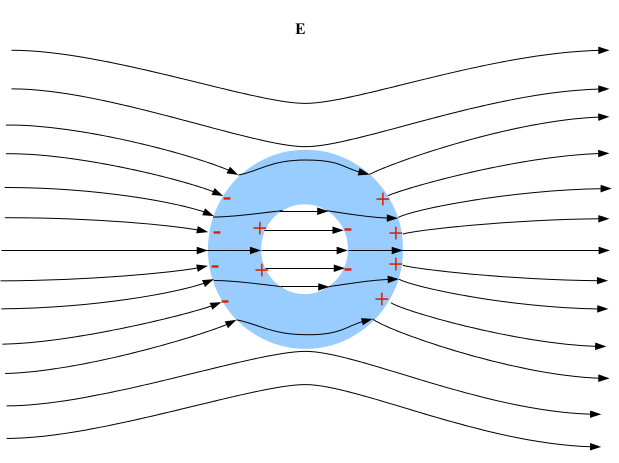
\includegraphics[scale=0.46]{problema3fig1}
 \caption{Gráfico del comportamiento del campo eléctrico para el caso $b\simeq 2a$. Notar 
 que la figura no la realicé completamente yo, la tome de 
 \href{http://bit.ly/1pslIha}{http://bit.ly/1pslIha} y 
 la modifiqué un poco.}
\end{figure}

\textbf{(c)} Para un cilindro dieléctrico sólido en un campo, solamente tenemos que 
hacer $a \rightarrow 0$, y tenemos 

\begin{equation}
 \boxed{\mathbf{E}_{\rho < b} = \frac{2\epsilon_0}{\epsilon + \epsilon_0}E_0 \hat{i}},
\end{equation}

\begin{equation}
 \boxed{ \mathbf{E}_{\rho > b} = E_0\hat{i} + \frac{(\epsilon - \epsilon_0)b^2}
 {(\epsilon + \epsilon_0)\rho^2}E_0(\hat{i} + 2\hat{\phi}\sen{\phi})}.
\end{equation}

Para una cavidad cilíndrica en un dieléctrico uniforme, solamente tenemos que 
hacer $b \rightarrow 0$, y obtenemos 

\begin{equation}
 \boxed{\mathbf{E}_{\rho < a} = \frac{3\epsilon\epsilon_0}{(\epsilon + \epsilon_0)^2}
 E_0 \hat{i}},
\end{equation}

\begin{equation}
 \boxed{\mathbf{E}_{\rho > a} = \frac{2\epsilon_0}{(\epsilon + \epsilon_0)^2}E_0 
 \left[(\epsilon + \epsilon_0)\hat{i} - (\epsilon - \epsilon_0)\frac{a^2}{\rho^2}
 (\hat{i} + 2\hat{\phi}\sen{\phi})\right]}.
\end{equation}

\newpage

\section{Problema 4. Problema 4.9 de Classical Electromagnetic Radiation
de Jackson \cite{jackson}.}

Una carga puntual $q$ es colocada en el espacio libre a una distancia $d$ del centro 
de una esfera dieléctrica de radio $a$ ($a < d)$ y constante dieléctrica 
$\epsilon/\epsilon_0$. 

\begin{enumerate}[label=\textbf{(\alph*)}]
\item Encuentre el potencial en todos los puntos del espacio como una expansión 
en armónicos esféricos.
\item Calcule las componentes rectangulares del campo eléctrico cerca del 
centro de la esfera.
\item Verifique que, en el límite $\epsilon/\epsilon_0 \rightarrow \infty$, tu 
resultado es el mismo que para la esfera conductora.
\end{enumerate}

\vspace{.3cm}

\underline{Solución:} \vspace{.3cm}

Si colocamos la esfera en el origen y la carga puntual en el eje $z$ a una distancia 
$z = d$ el problema tendrá simetría azimutal, y por lo tanto $m = 0$ y la solución 
puede expresarse en términos de los polinomios de Legendre, lo cual será más simple 
que en armónicos esféricos, y no se pierde generalidad con esta suposición. 

\begin{figure}[H]
 \center 
 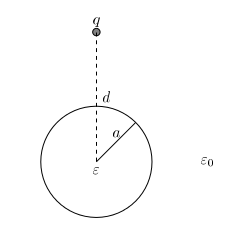
\includegraphics[scale=0.8]{problema4fig1}
 \caption{Geometría asumida para el sistema del problema 4.}
\end{figure}


Debemos resolver el problema para las dos regiones, y utilizar las condiciones 
de frontera para así encontrar una solución completa. Tenemos las siguientes dos 
regiones:

\begin{equation}
 \Phi_{r < a} \quad \qquad \text{donde tenemos } \epsilon,
\end{equation}

\begin{equation}
  \Phi_{r > a} \quad \qquad \text{donde tenemos } \epsilon_0.
\end{equation}

Resolvamos primero la región $r > a$ utilizando el método de imágenes. Para esto 
colocamos una carga imagen $q'$ en $z = a^2/d$ para dar cuenta de los efectos 
de la esfera dieléctrica, y la posición que hemos escogido ha sido basada en 
los resultados obtenidos en la sección 2.2 de Jackson \cite{jackson}, específicamente 
la ecuación (2.4). El potencial en la región exterior debido a la carga puntual 
y la carga imagen es 

\begin{equation}
 \Phi_{r > a} = \frac{1}{4\pi\epsilon_0}\left(\frac{q}{|\mathbf{r}-d\hat{z}|} 
 + \frac{q'}{|\mathbf{r} - (a^2/d)\hat{z}|}\right),
\end{equation}

ahora expandiendo en series de polinomios de Legendre y combinando

\begin{equation}
 \frac{1}{|\mathbf{r} - \mathbf{r}_0} = 
 \sum_{l=0}^\infty \frac{r_{>}^l}{r_{<}^{l+1}}P_l(\cos{\theta}),
\end{equation}

donde $r_{<}$ es el más pequeño entre $(r,r_0)$. Entonces si $r > d$ 

\begin{equation}
 \Phi_{r > a} = \frac{1}{4\pi\epsilon_0}\sum_{l=0}^\infty P_l(\cos{\theta} 
 \frac{1}{r^{l+1}} \left(qd^l + q'\frac{a^{2l}}{d^l}\right),
\end{equation}

y si $r < d$

\begin{equation}
  \Phi_{r > a} = \frac{1}{4\pi\epsilon_0}\sum_{l=0}^\infty P_l(\cos{\theta} 
  \left(q\frac{r^l}{d^{l+1}} + q'\frac{a^{2l}}{d^lr^{l+1}} \right).
\end{equation}

Resolvamos ahora para el potencial adentro de la esfera. Ya que no hay carga adentro 
de la esfera, solo necesitamos una carga imagen $q''$ afuera de la esfera en $z=d$ 
para simular los efectos de el material dieléctrico. Tenemos entonces 

\begin{equation}
 \Phi_{r < a} = \frac{1}{4\pi\epsilon}\left(\frac{q''}{|\mathbf{r} - d\hat{z}|}\right). 
\end{equation}

Ahora ya que $r$ siempre es más pequeño que $d''$, solo necesitamos una expansión 

\begin{equation}
 \Phi_{r < a} = \frac{1}{4\pi\epsilon}\left(\sum_{l=0}^\infty q'' 
 \frac{r^l}{d^{l+1}}P_l(\cos{\theta})\right).
\end{equation}

Para encontrar expresiones para $q'$ y $q''$ debemos aplicar la condición de 
frontera en $r = a$ que nos dice que $(\mathbf{D}_2 
- \mathbf{D}_1)\cdot n_{12} = \sigma$, y debido a que no hay densidad de carga 
libre en la superficie de la esfera, esta condición se convierte en\footnote{Donde 
estamos usando el hecho de que $\mathbf{D} = \epsilon \mathbf{E}$ en este caso.}

\begin{equation}
 \left(\epsilon_0 \mathbf{E}_{r > a} - \epsilon \mathbf{E}_{r < a}\right)\cdot \hat{r} = 0,
\end{equation}

que implica usando la definición de campo eléctrico dado el potencial eléctrico 

\begin{equation}
 \epsilon_0 \frac{\partial \Phi_{r > a}}{\partial r} = \epsilon 
 \frac{\partial \Phi_{r < a}}{\partial r},
\end{equation}

y derivando obtenemos 

\begin{equation}
 \boxed{ql + q'(-l -1)\frac{d}{a} = q'' l}.
\end{equation}

Aplicando la segunda condición de frontera en $r = a$ que nos dice que 
$(\mathbf{E}_2 - \mathbf{E}_1) \times \mathbf{n}_{12} = 0$ tenemos 

\begin{equation}
 \left\zerodel E_{r < a}\right|_\theta = \left\zerodel E_{r > a}\right|_\theta,
\end{equation}

\begin{equation}
 \therefore \frac{\partial \Phi_{r > a}}{\partial r} = 
 \frac{\partial \Phi_{r < a}}{\partial r},
\end{equation}

y derivando encontramos 

\begin{equation}
 \boxed{q'' = \frac{\epsilon}{\epsilon_0}q + \frac{\epsilon}{\epsilon_0}q'\frac{d}{a}}.
\end{equation}

Resolviendo las ecuaciones en cajas con \texttt{Mathematica$^\circledR$} encontramos 

\begin{equation}
 q' = \frac{\frac{\epsilon_0}{\epsilon} - 1}{d\left[\frac{\epsilon_0}{\epsilon}(l+1) + l\right]},
\end{equation}

y 

\begin{equation}
 q'' = \frac{q(2l + 1)}{\frac{\epsilon_0}{\epsilon}(l+1) +l}.
\end{equation}

Podemos escribir el resultado final para los potenciales como 

\begin{equation}
 \boxed{\Phi_{r < a} = \frac{q}{4\pi\epsilon d}\left[\sum_{l=0}^\infty 
 \frac{q(2l + 1)}{\frac{\epsilon_0}{\epsilon}(l+1) +l} \left(\frac{r}{d}\right)^l
 P_l(\cos{\theta})\right]},
\end{equation}

\begin{equation}
 \boxed{\Phi_{r > a} =  \frac{q}{4\pi\epsilon d}\sum_{l=0}^\infty P_l(\cos{\theta})
 \frac{d^{l+1}}{r^{l+1}}\left[1 +  \frac{l\left(\frac{\epsilon_0}{\epsilon} - 1\right)}{\left[\frac{\epsilon_0}{\epsilon}(l+1) + l\right]}
 \left(\frac{a}{d}\right)^{2l+1}\right] \qquad \text{si } r > d},
\end{equation}

\begin{equation}
 \boxed{\Phi_{r > a} =  \frac{q}{4\pi\epsilon d}\sum_{l=0}^\infty P_l(\cos{\theta})
 \left[\left(\frac{r}{d}\right)^l +  \frac{l\left(\frac{\epsilon_0}{\epsilon} - 1\right)}{\left[\frac{\epsilon_0}{\epsilon}(l+1) + l\right]}
 \left(\frac{a}{d}\right)^{l}\left(\frac{a}{r}\right)^{l+1}\right] \qquad \text{si } r < d}.
\end{equation}

\textbf{(b)} Cerca del centro de la esfera tenemos $r \ll d \rightarrow r/d \ll 1$. 
Debido a que el campo interno está en términos de potencias de $r/d$, los órdenes 
superiores pueden despreciarse 

\begin{equation}
 \Phi_{r \ll d} = \frac{q}{4\pi\epsilon_0 d}\left[1 + \frac{3}{1+2\epsilon_0/\epsilon}
 \frac{r}{d}\cos{\theta}\right],
\end{equation}

que podemos escribir como 

\begin{equation}
 \Phi_{r \ll d} = \frac{q}{4\pi\epsilon_0 d}\left[1 + \frac{3}{2 + \epsilon/\epsilon_0}
 \frac{z}{d}\right].
\end{equation}

El campo eléctrico lo calculamos con 

\begin{equation}
 \mathbf{E}_{r \ll d} = -\nabla \Phi_{r \ll d},
\end{equation}

que resulta en 

\begin{equation}
 \boxed{\mathbf{E}_{r \ll d} = - \frac{q}{4\pi\epsilon_0 d^2}\left[\frac{3}{2 + 
 \epsilon/\epsilon_0}\right] \hat{z}}.
\end{equation}

El campo eléctrico cera del centro de la esfera apunta haca el lado contrario 
de la carga puntual, en la dirección negativa del eje $z$.

\vspace{.3cm}

\text{(c)} En el límite en que $\epsilon/\epsilon_0$, vemos que todos los términos 
de la serie se hacen cero menos el término con $l=0$, entonces 

\begin{equation}
 \boxed{\Phi_{r < a} = \frac{q}{4\pi\epsilon_0d}},
\end{equation}

exactamente lo que encontramos para una esfera conductora. Y el otro caso, comenzamos 
por reescribir $\Phi_{r > a}$ como 

\begin{equation}
 \Phi_{r > a} = \frac{q}{4\pi\epsilon_0}\frac{a}{rd} + \frac{q}{4\pi\epsilon_0} 
 \sum_{l=0}^\infty \frac{r_{<}^l}{r_{>}^{l+1}}P_l(\cos{\theta}) - 
 \frac{qa}{4\pi\epsilon_0}\sum_{l=0}^\infty \frac{a^{2l}}{(rd)^{l+1}}P_l(\cos{\theta}),
\end{equation}

pero según la ecuación (3.38) de Jackson \cite{jackson}

\begin{equation}
  \sum_{l=0}^\infty \frac{r_{<}^l}{r_{>}^{l+1}}P_l(\cos{\theta}) = 
  \frac{1}{|\mathbf{r} - d\mathbf{z}|},
\end{equation}

y 

\begin{equation}
 \sum_{l=0}^\infty \frac{a^{2l}}{(rd)^{l+1}}P_l(\cos{\theta}) = 
 \frac{1}{|a^2\mathbf{z} - d\mathbf{r}|},
\end{equation}

por lo tanto 

\begin{equation}
 \boxed{\Phi_{r > a} = \frac{q}{4\pi\epsilon_0}\left[\frac{a}{rd} + 
 \frac{1}{|\mathbf{r} - d\mathbf{z}|} -
  \frac{a/d}{|\frac{a^2}{d}\mathbf{z} - d\mathbf{r}|}\right]},
\end{equation}

que también tiene la misma forma que la ecuación (2.8) de Jackson \cite{jackson} 
donde se calcula este potencial.

\hspace{10cm}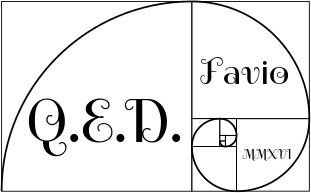
\includegraphics[scale=0.25]{logoQED}

\newpage

\section{Problema 5. Problema 4.13 de Classical Electromagnetic Radiation
de Jackson \cite{jackson}.}

Dos superficies cilíndricas conductoras, largas y coaxiales, de radios $a$ y $b$ 
son bajadas verticalmente a un líquido dieléctrico. Si el líquido sube una altura 
promedio de $h$ entre los electrodos cuando una diferencia de potencial $V$ es 
establecida entre ellos, muestre que la susceptibilidad del líquido es\footnote{Hemos 
cambiado la letra usada para la densidad por conveniencia.}

$$
\chi_e = \frac{(b^2 - a^2)\xi g h \ln{(b/a)}}{\epsilon_0 V^2}
$$

donde $\xi$ es la densidad del líquido, $g$ es la aceleración debida a la gravedad, 
y la susceptibilidad del aire es depreciada.

\vspace{.3cm}

\underline{Solución:} \vspace{.3cm}

Hay dos regiones que considerar en este problema, una entre los cilindros con aire 
y la otra entre los cilindros con agua. Aunque existan dos permitividades distintas, 
el campo $\mathbf{D}$ debe ser el mismo en las dos regiones. Por conveniencia colocaremos 
el eje del cilindro en el eje $z$, y debido a que el cilindro es largo, podemos 
ignorar la dimensión $z$ y podemos resolver la ecuación de Laplace en dos dimensiones. 
Recordemos que esta tiene la forma\footnote{Ver ecuación (2.71) de Jackson \cite{jackson}.}

\begin{equation}
 \Phi(\rho,\phi) = a_0 + b_0 \ln{\rho} + \sum_{m=1}^\infty (a_m \rho^m + b_m \rho^{-m})
 (A_m \euler^{im\phi} + B_m \euler^{-im\phi}).
\end{equation}

Y ya que el problema tiene simetría azimutal, esta ecuación se reduce a 

\begin{equation}
 \Phi(\rho,\phi) = a_0 + b_0 \ln{\rho}.
\end{equation}

Si asumimos ahora que la diferencia de potencial $V$ establecida entre las superficies 
cilíndricas conductoras es tal que en la de adentro es cero el potencial, y en la 
de afuera es $V$, tenemos que 

\begin{equation}
 \Phi(\rho = a) = 0,
\end{equation}

\begin{equation}
 0 = a_0 + b_0\ln{a},
\end{equation}

\begin{equation}
 \therefore q_0 = - b_0 \ln_a,
\end{equation}

y la solución se convierte por ahora en (utilizando las propiedades de los logaritmos)

\begin{equation}
 \Phi(\rho,\phi) = b_0 \ln({\rho/a}),
\end{equation}

para obtener la forma de $b_0$ hacemos, 

\begin{equation}
 \Phi(\rho = b) = V,
\end{equation}

\begin{equation}
 V =  b_0 \ln({\rho/a}),
\end{equation}

\begin{equation}
 \therefore b_0 = \frac{V}{\ln{(b/a)}}.
\end{equation}

Y el potencial es entonces 

\begin{equation}
 \Phi(\rho,\phi) = V \frac{\ln{(\rho/a)}}{\ln{(b/a)}}.
\end{equation}

El campo eléctrico será 

\begin{equation}
 \mathbf{E} = -\nabla \Phi = - V \frac{1}{\ln{(b/a)}}\frac{1}{\rho} \hat{\rho}.
\end{equation}

Ahora, debido a que se debe conservar la energía, la energía potencial $W$ que 
había cuando la región entre los cilindros estaba completamente llena de aire y
la energía potencial después que se introducen los cilindros en el agua y se llega 
al equilibrio $W'$, debe ser tal que se mantenga la diferencia de potencial $V$ 
entre ellos, es decir que debe proveerse energía externa al sistema para mantener 
el potencial mientras el sistema cambia. Tenemos entonces 

\begin{equation}
 \Delta W = W' - W,
\end{equation}

y recordando que en materiales $W = \frac{1}{2}\int \mathbf{E}\cdot \mathbf{D} d^3x$
tenemos\footnote{Los primados se refieren a luego de introducidos en el líquido.}

\begin{equation}
 \Delta W = \frac{1}{2}\int \mathbf{E}'\cdot \mathbf{D}' d^3 \mathbf{x} - 
 \frac{1}{2}\int \mathbf{E}\cdot \mathbf{D} d^3 \mathbf{x},
\end{equation}

y ya que esta ecuación debe depender de las propiedades del líquido en que 
las superficies cilíndricas son introducidas podemos escribir esta ecuación 
como\footnote{Ver ecuación (4.38) de Jackson \cite{jackson}.}

\begin{equation*}
 \Delta W = \left[\frac{1}{2}(L -h)\epsilon_0  \int E_{\text{aire}}^2 d^2 \mathbf{x} 
 +  \frac{1}{2}h\epsilon_0(1 + \chi_e)h \int E_{\text{líquido}}^2 d^2 \mathbf{x} 
 \right] - \left[\frac{1}{2}L\epsilon_0\int E_{\text{aire}}^2 d^2 \mathbf{x} \right]
\end{equation*}

donde $L$ es la longitud de los cilindros. Esta ecuación se reduce a 

\begin{equation}
 \therefore \Delta W = \frac{1}{2}h\epsilon_0 \int E_{\text{aire}}^2 d^2 \mathbf{x} +
 \frac{1}{2}h\epsilon_0(1 + \chi_e)h \int E_{\text{líquido}}^2 d^2 \mathbf{x}.
\end{equation}

Y ya que el campo eléctrico debe ser el mismo en las dos regiones tenemos 

\begin{equation}
 \Delta W = \frac{h\epsilon_0 \chi_e}{2}\int E^2 d^2\mathbf{x},
\end{equation}

\begin{equation}
 \therefore \Delta W = \frac{h\epsilon_0 \chi_e}{2}2\pi \int_a^b E^2 \rho d\rho,
\end{equation}

e introduciendo la expresión para el campo eléctrico que obtuvimos 

\begin{equation}
 \therefore \Delta W = \frac{h\epsilon_0 \chi_e}{2}2\pi \int_a^b 
 \left(V^2 \frac{1}{\ln^2{(b/a)}}\frac{1}{\rho^2} \right)\rho d\rho,
\end{equation}

e integrando obtenemos 

\begin{equation}
  \Delta W = \frac{\pi h \epsilon_0 \chi_e V^2}{\ln^2{(b/a)}}.
\end{equation}

Esta es la energía potencial ganada en los campos resultante de introducir las 
superficies cilíndricas en el líquido dieléctrico a una altura $h$. También podemos 
ver el cambio de energía potencial como una energía potencial gravitacional, en 
este caso 

\begin{equation}
 \Delta W = mhg,
\end{equation}

y usando la definición de densidad $\xi = m/V$ podemos escribir 

\begin{equation}
 \Delta W = \xi h A gh,
\end{equation}

pero el área $A = \pi(b^2 - a^2)h$, 

\begin{equation}
 \therefore \Delta W = \xi \pi(b^2 - a^2)h^2 g,
\end{equation}

Ahora claramente estas dos diferencias de energía cinética deben ser iguales, por lo 
tanto 

\begin{equation}
  \frac{\pi h \epsilon_0 \chi_e V^2}{\ln^2{(b/a)}} = \xi \pi(b^2 - a^2)h^2 g,
\end{equation}

y resolviendo para $\chi_e$ encontramos 

\begin{equation}
 \boxed{\chi_e = \frac{(b^2 - a^2)\xi g h \ln{(b/a)}}{\epsilon_0 V^2}}.
\end{equation}

\hspace{10cm}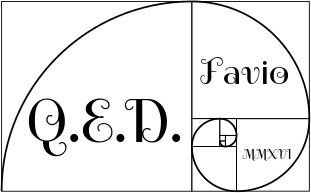
\includegraphics[scale=0.25]{logoQED}

\newpage

\begin{thebibliography}{10}
\bibitem{jackson}
J. Jackson, \emph{Classical Electrodynamics}, 3ra edición. John Wiley and Sons, Inc. 
1999.
\bibitem{marion2}
J. Marion, M. Heald, \emph{Classical Electromagnetic Radiation}, 2da edición, Academic 
Press, 1965.
\end{thebibliography}

\end{document}